\chapter{Referencial Teórico}
\label{ref}
\section{Software Analytics}
\label{ref:sof}
Durante muito tempo, a falta de dados em projetos de software foi uma constante.
Agora com o auxílio da internet e dos projetos de software livre, existem tantos
dados relacionados a projetos de software que é manualmente impossível de analisá-los
por completo\cite{artAndScience}. Ao fim de 2012, pesquisas mostraram que o \textit{Mozilla Firefox} 
teve 800.000 relatos de bugs e outras plataformas como \textit{Sourcefoge.net}
e o \textit{Github} hospedam 324.000 e 11.2 milhões de projetos, respectivamente\cite{informationNeeds}.

Para ser capaz de manipular essa grande quantidade de dados, muitos pesquisadores
se voltaram para o uso e \textit{analytics}, ou seja, o uso de análises, dados e
raciocínio sistemático para tomar decisões. Podemos definir \textit{Software Analytics}
como: `A análise de dados de software para gerentes e engenheiros de software, 
com o objetivo de capacitar indivíduos e times de desenvolvimento, a ganhar e difundir 
conhecimento a partir de seus dados para tomar melhores decisões'\cite{informationNeeds}.

Hoje é comum empresas como Google, Facebook e Microsoft aplicarem métodos de data
science diariamente em seus projetos. Além disto, o número de conferencias neste
tópico aumentou bastante, sendo as duas mais importantes \textit{Mining Software
Repositories} (MSR) e a \textit{PROMISE Conference on Repeatable Experimentes in Software
Engineering}, cada uma com um foco diferente, sendo a MSR preocupada com a coleta dos dados
enquanto a PROMISE com a eficacia e repetibilidade da análise de dados.

As metodologias ágeis, acompanhando o crescimento da utilização do Data Science no
mercado, também vem utilizando desta técnica para otimizar a evolução de produto. Um
dos meios de aplicar a análise de dados em um ciclo ágil é utilizar uma abordagem 
analítica de planejamento de release, ou seja utilizar fontes externas e internas
de dados para planejar as entregas futuras do produto de software. 

A análise de dados obtidos de ferramentas de versionamento de código, como o Git,
Bazaar, Subversion ou CVS podem trazer informações importantes a respeito da evolução
de um projeto de software, do nível de engajamento dos desenvolvedores, número de defeitos
e do desenvolvimento distribuído e muitos outros tópicos\cite{artAndScience}. O Github,
uma das ferramentas mais utilizadas de versionamento de código, fornece uma api que permite
a extração de dois tipos de dados:

\begin{itemize}
\item \textbf{Metadados:} Os metadados fornecidos são informações associadas a cada
commit ou issue, são elas: criador(a), data, mensagem do commit ou issue, a branch e repositório,
e o escopo do commit ou issue. Além disto, na mensagem do commit podem haver referencias a outros
desenvolvedores, bugs ou outros commits e issues.
\item \textbf{Snapshots:} O código fonte do projeto, que pode ser obtido em diferentes
fases do desenvolvimento, já que a ferramente permite que um usuário avance ou retroceda
dentro dos commits. Desta forma, é possível analisar o código de um projeto referente
a vários períodos diferentes.
\end{itemize}

Abaixo, na figura~\ref{fig:github_api}, podemos ver o digrama de classes da API fornecida pelo
Github, com base nesta imagem, é possível ver que as issues e informações dos commiters
são exportadas a partir de um ponto comum de acesso.

\begin{figure}[h]
    \centering
        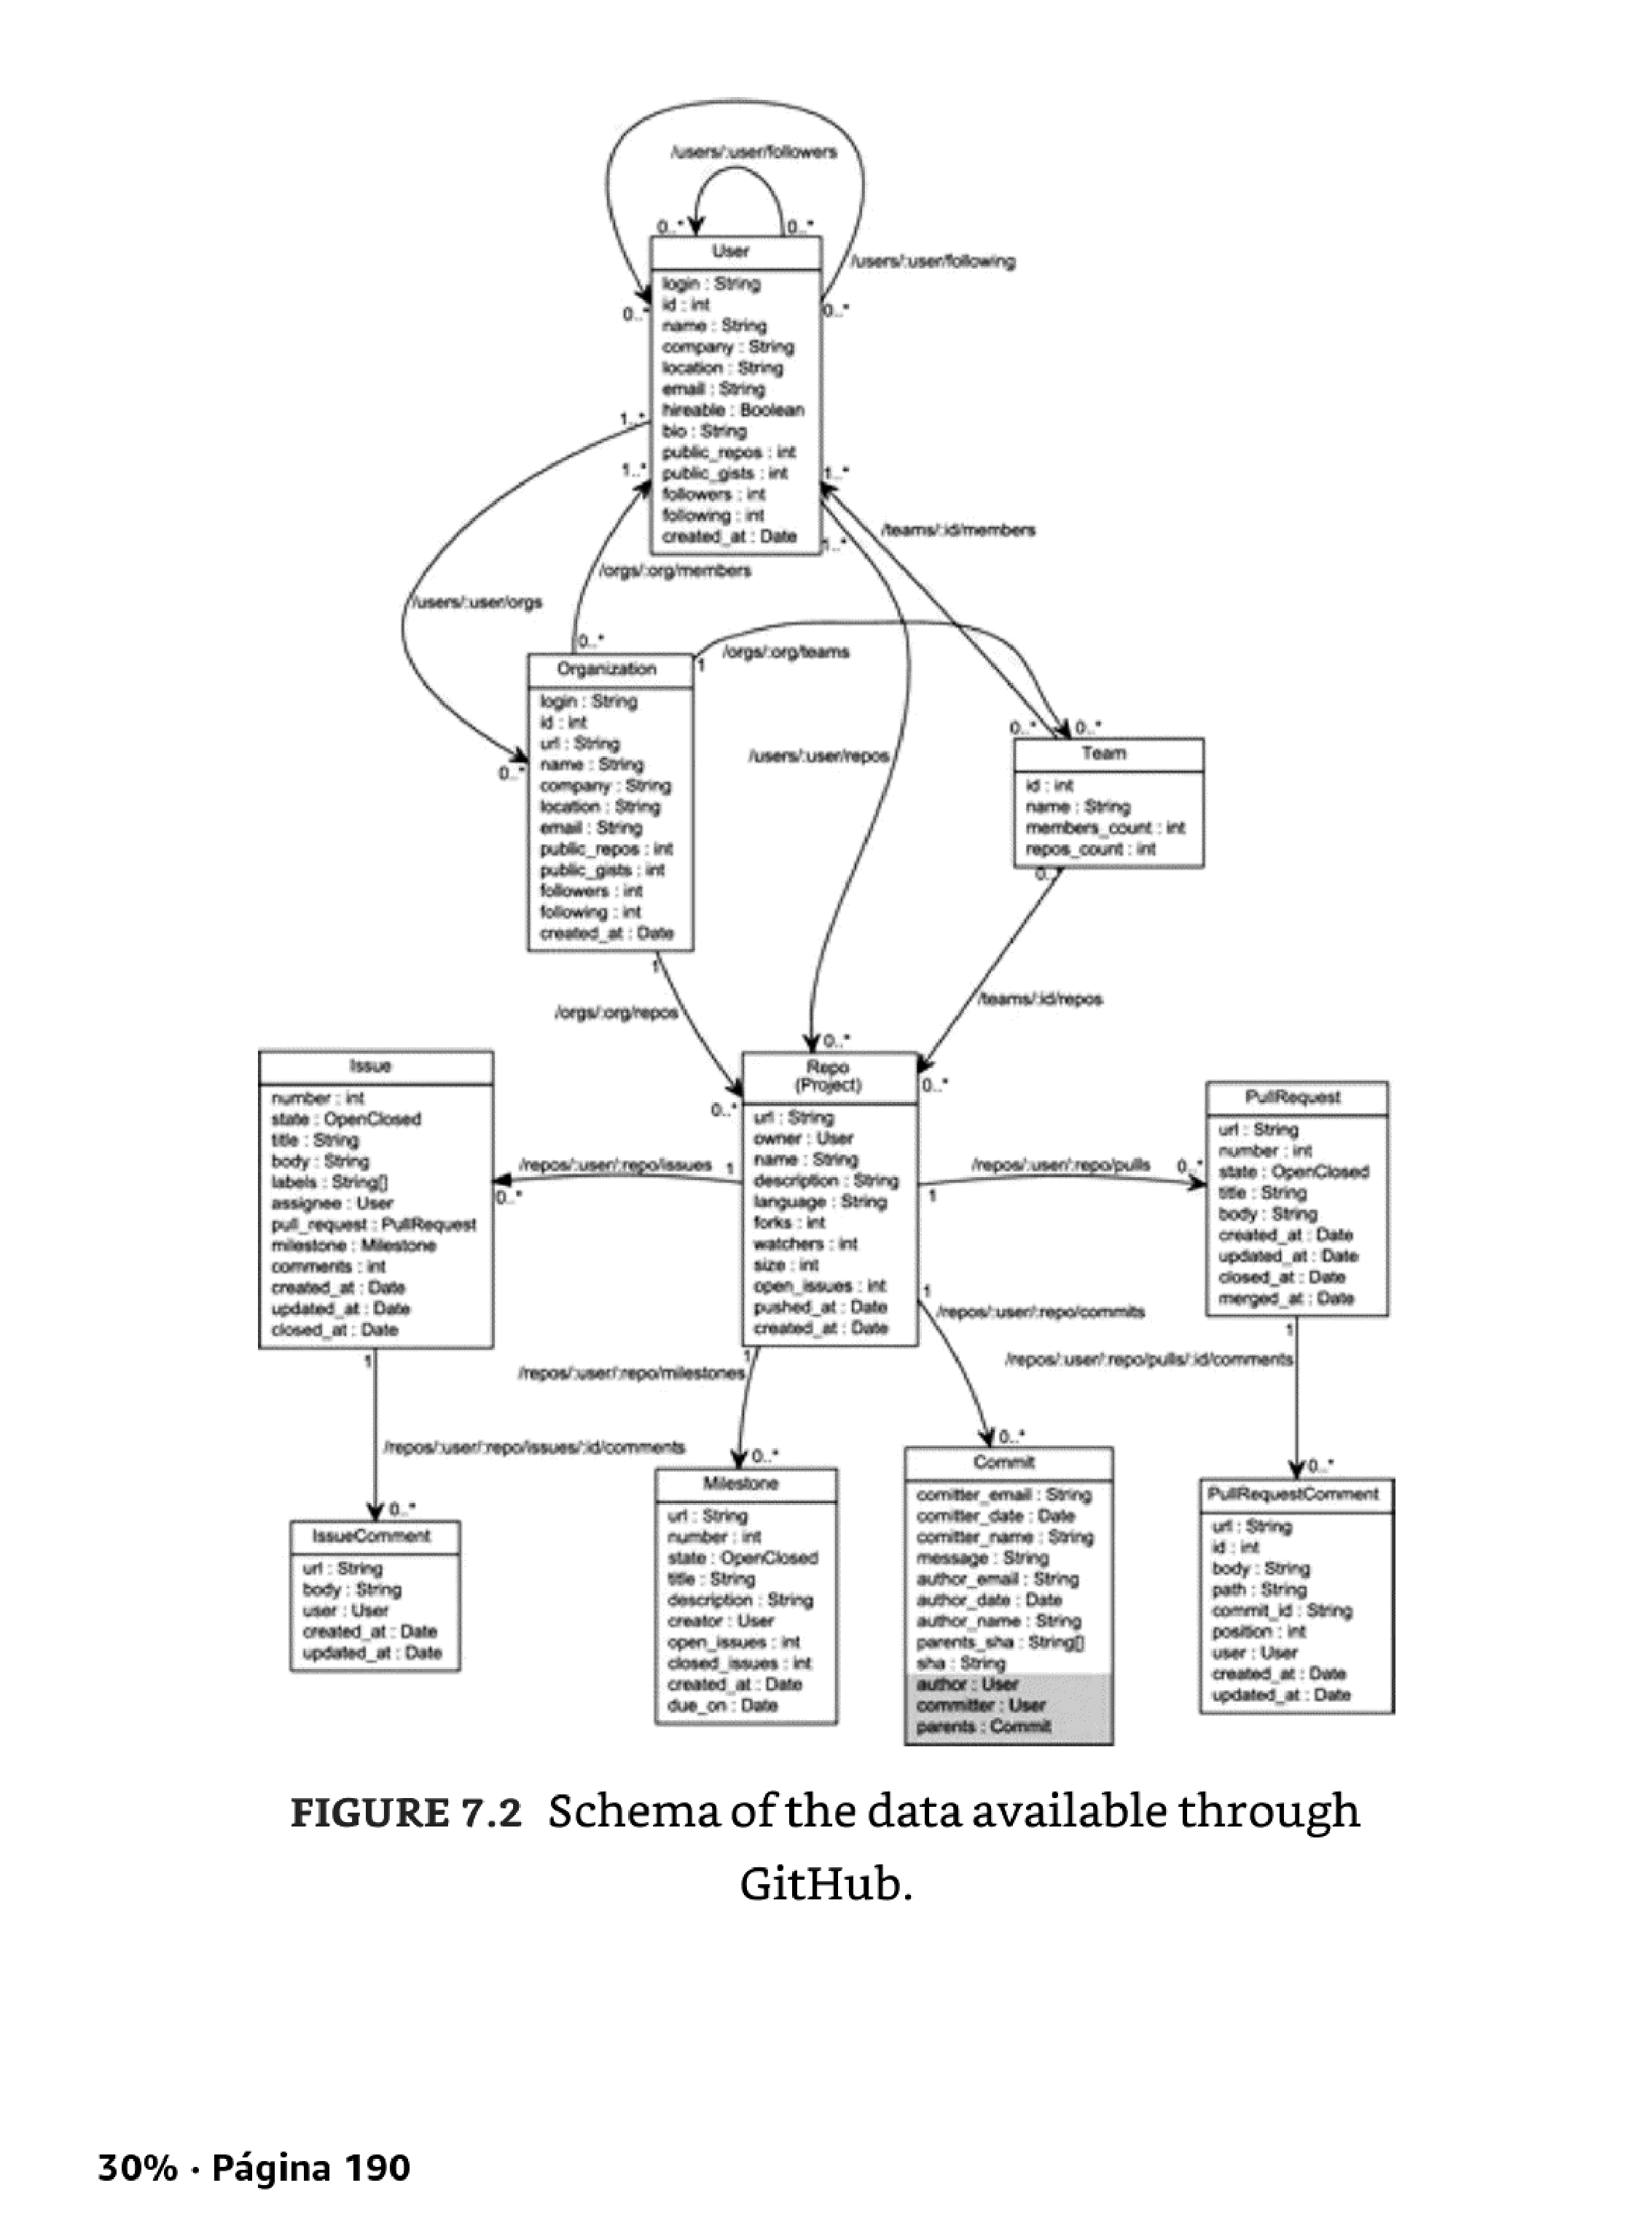
\includegraphics[keepaspectratio=true,scale=0.3]{figuras/github_api_diagram.eps}
    \caption{Representação UML da API do Github}
    \label{fig:github_api}
\end{figure}

Utilizando-se das informações mostradas na figura~\ref{fig:github_api} é possível utilizar
\textit{Software Analytics} para possibilitar uma melhor tomada de decisão em um
repositório que utilize da ferramenta Github para organizar o trabalho.

\section{Centralidade de Redes}
\label{ref:cen}
Centralidade é um dos tópicos mais estudados na análise de redes sociais, ele 
determina o grau de importância de um vértice dentre todos os outros dentro de uma 
rede, a figura~\ref{fig:centrality} apresenta um exemplo de centralidade. 
O conceito de centralidade de redes já foi aplicado a diversos contextos, dentre eles: investigar a influencia 
de redes inter organizacionais, estudos de relevância, vantagens em redes de troca, 
competência em organizações formais, oportunidades de emprego e diversos outros campos 
do mercado e ciência\cite{centrality}.

\begin{figure}[h]
    \centering
        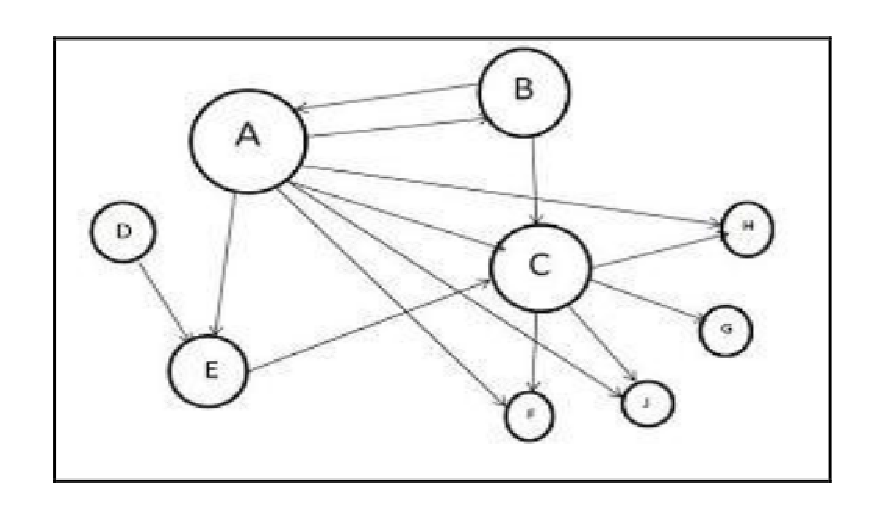
\includegraphics[keepaspectratio=true,scale=0.5]{figuras/centrality.eps}
    \caption{Exemplificação de Relevância de um Nó em uma Rede}
    \label{fig:centrality}
\end{figure}

Diversos processos comumente encontrados no dia-a-dia são processos de fluxo. Estes
processos diferem em dimensão e tipo, mas ainda assim podem ser comparados e exemplificados.
Abaixo é possível ver alguns desses processos e como eles podem ser descritos em uma perspectiva
da Teoria dos Grafos\cite{ceflow}.  

\begin{itemize}
\item Dinheiro: Considere uma moeda, ou nota de um dólar, que se move pela
economia e muda de mãos a cada transação. Uma nota é indivisível e só pode estar
em um lugar em um determinado período de tempo. Em uma perspectiva de teoria dos
grafos, a movimentação de uma nota em uma rede pode ser feita como um \textit{passeio (Walk)},
sendo, desta forma, representado como um processo de Markov
\item Fofoca: Imagine uma informação privada que passa por uma rede
de empregados de uma empresa. Diferentemente de uma nota, essa mesma informação
pode estar em diversos locais diferentes em um determinado período de tempo, se
replicando a cada pessoa que passa a ter acesso a informação, mas geralmente
não atravessa o mesmo vértice mais que uma vez, apesar de poder visitar o mesmo nó
mais de uma vez. A movimentação desta informação em grafo pode ser representada como
uma trilha.
\item E-mail: Um vírus, o spam de e-mail, que envia mensagens a todos os
contatos de uma pessoa simultaneamente pode ser considerado um processo de fluxo.
Um e-mail pode ser representado como uma trilha da mesma forma que é realizado 
com uma informação, já que compartilham de características bem parecidas, como 
existir em diversos locais ao mesmo tempo, e geralmente, os e-mails não passarem
pelo mesmo vértice, ou caminho, duas vezes.
\item Infecções: O caso de uma infecção em que o hospedeiro ficou imune.
A infecção vão passar por duplicação de pessoa a pessoa, mas nunca vai voltar a infectar
aqueles que já se tornaram imunes.
\item Pacotes: Um pacote de rede, que possui a característica de possuir
um remetente e um destinatário. Normalmente é preferível que o pacote tome o menor
caminho possível até chegar ao seu destino, desta forma a movimentação do pacote
deve seguir o caminho geodésico pela rede e roteadores. 
\end{itemize}

Durante os anos, muitos métodos de medida de centralidade foram criados, entre eles:
Centralidade de Grau, Proximidade \textit{(Closeness)}, Intermediação \textit{(Betweenness)}, 
Autovetor \textit{(Eigen Vector)}, Informação, Intermediação de Fluxo, \textit{Rush Index},
Medidas de Influencia de Katz, Hubbell, Hoede e Taylor. Estes métodos diferem nas suposições
iniciais que fazem para alcançar o objetivo de determinar o nó com maior importância, por exemplo,
o algoritmo de Freeman de proximidade e intermediação conta apenas os caminhos geodésicos entre 
os nós, assumindo que qualquer fluxo que percorra uma rede, siga sempre pelo caminho mais curto.
Outros algoritmos como a centralidade de autovetor de Bonacich conta travessias, o que assume
que as trajetórias podem ser sinuosas, atravessando nós e arestas repetidas vezes até chegar ao
destino\cite{centrality}.

\section{Ranqueamento de Páginas}
\label{ref:ran}
O algoritmo de ranqueamento de páginas foi inventado por Larry Page e Sergey em
1996, ele permite calcular a importância relativa de páginas da web e tem aplicações
em mecanismos de busca, estimativas de trafego e navegação na web. Ele foi criado
com o intuito de prover uma solução de busca de informações na web e aproveitar
a estrutura de de links, usada no hipertexto da web, possui\cite{pageRank}.

A premissa do algoritmo de ranqueamento de páginas é que cada página na web
possui um número de links de saída e de entrada, e que páginas com um grande
número de links são mais importantes do que as com poucos links. Além disto,
o algoritmo também leva em consideração a relevância dos links de entrada
de uma página, ou seja, se uma página da web possui um link de entrada que
possui uma alta relevância, essa página tende a ser mais importante que outra
que possua vários links mas que vieram de lugares mais obscuros. A imagem~\ref{fig:page_rank}
exemplifica como a relevância de uma página influencia as páginas seguintes.

\begin{figure}[h]
    \centering
        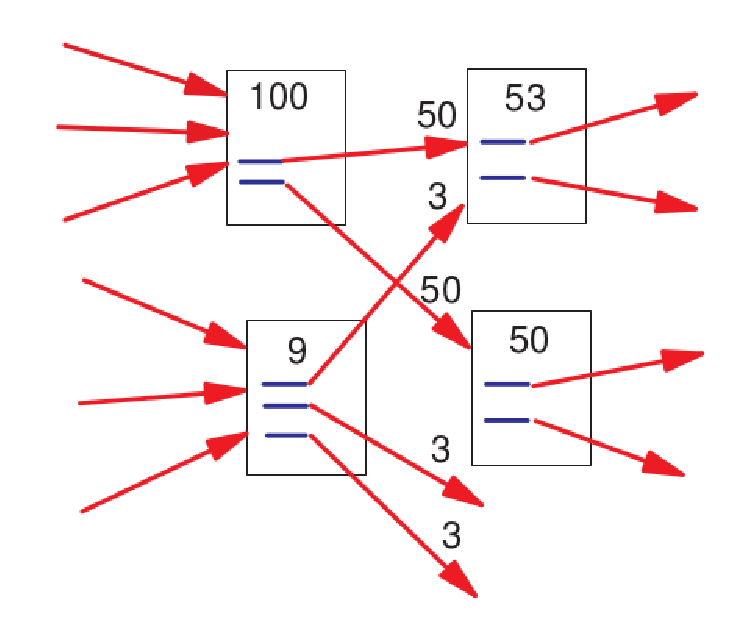
\includegraphics[keepaspectratio=true,scale=0.5]{figuras/page_rank.eps}
    \caption{Simplificação do Cálculo de Ranqueamento de Páginas}
    \label{fig:page_rank}
\end{figure}

\begin{figure}[h]
    \centering
        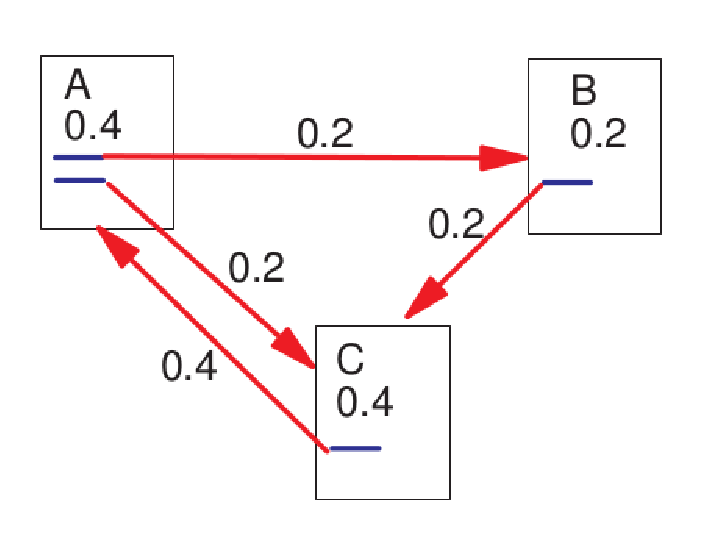
\includegraphics[keepaspectratio=true,scale=0.5]{figuras/page_rank2.eps}
    \caption{Simplificação do Cálculo de Ranqueamento de Páginas}
    \label{fig:page_rank2}
\end{figure}

A figura~\ref{fig:page_rank} mostra como o ranqueamento de páginas se divide através
das paginas e como ele contribui para o ranque das páginas seguintes. Já a 
figura~\ref{fig:page_rank2} mostra como um estado estável pode ser alcançado
depois que o algoritmo é executado em um conjunto de páginas. 

\begin{figure}[h]
    \centering
        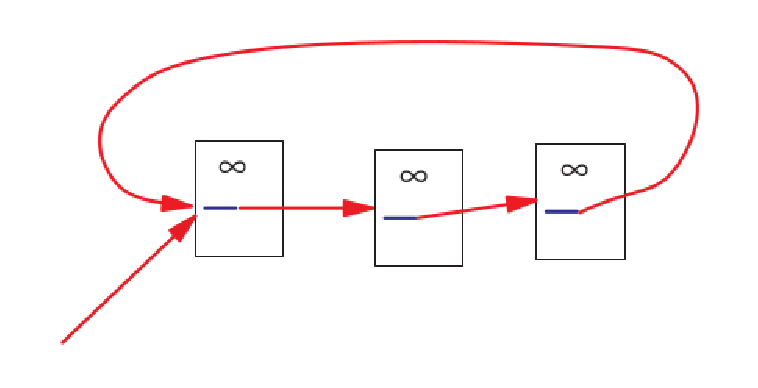
\includegraphics[keepaspectratio=true,scale=0.5]{figuras/page_rank3.eps}
    \caption{Loop de Ranqueamento}
    \label{fig:page_rank3}
\end{figure}

Um dos problemas dessa função de ranqueamento, é que caso duas páginas da web que apontem uma para
outra, e uma terceira aponte para qualquer uma destas, o loop vai acumular ranque
porém nunca vai distribuir isso para nenhuma outra página seguinte, é possível
ver esse fenômeno na figura~\ref{fig:page_rank3}.

Desta forma, a função de ranqueamento de páginas foi definida na seguinte forma:

Seja $x$ uma página da web. Então
\begin{itemize}
    \item $L(x)$ é o conjunto de websites que possuem link para $x$
    \item $C(y)$ é o grau de entrada de $y$
    \item $\alpha$ é a probabilidade de um pulo aleatório
    \item $N$ é o número total de websites
\end{itemize}
\[\displaystyle PR(x) := \alpha \left ( \frac{1}{N} \right ) + (1-\alpha) \sum_{y\in L(x)} \frac{PR(y)}{C(y)}\]

Aplicando a equação acima, é possível obter o ranque de uma página, dado um conjunto
de web-sites avaliados.
